

\usetikzlibrary{decorations.pathmorphing}
\usetikzlibrary{decorations.text}
\tikzset{
cross/.style={cross out, draw=black, minimum size=2*(#1-\pgflinewidth), inner sep=0pt, outer sep=0pt},
%     %default radius will be 1pt. 
cross/.default={3.5pt}
dot/.style={circle, fill=#1, inner sep=0, minimum size=4pt},
mini dot/.style={circle, inner sep=0pt, minimum size=2pt, pos=1, fill, node contents={}},
}

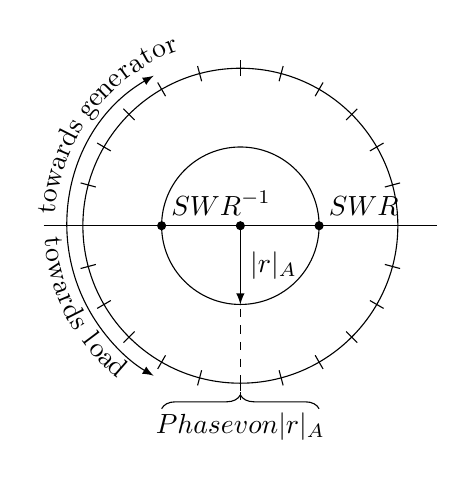
\begin{tikzpicture}
    \draw[-latex](0,0)--(0,-1) node[right, midway]{$|r|_A$};
    \draw[dashed](0,0)--(0,-2.25) node[below]{$\text{Phase von }|r|_A$};
    \draw [black,
        decorate,
        decoration = {brace,
                raise=5pt,
                amplitude=5pt}] (-1,-2.5) --  (1,-2.5);

    \draw[-,fill=black!100] (-1,0) circle (0.05) node[above right]{$\text{\tiny{SWR}}^\text{\tiny{-1}}$};
    \draw[-,fill=black!100] (0,0) circle (0.05);
    \draw[-,fill=black!100] (1,0) circle (0.05) node[above right]{$\text{\tiny{SWR}}$};
    \path (0,0) coordinate (c);
    \draw[-](-2.5,0)--(2.5,0);
    \node[, rotate around={85:(c)}] at (0,2.47){t};
    \node[, rotate around={81:(c)}] at (0,2.44){o};
    \node[, rotate around={76:(c)}] at (0,2.43){w};
    \node[, rotate around={71:(c)}] at (0,2.43){a};
    \node[, rotate around={67:(c)}] at (0,2.43){r};
    \node[, rotate around={63:(c)}] at (0,2.48){d};
    \node[, rotate around={59:(c)}] at (0,2.43){s};

    \node[, rotate around={53:(c)}] at (0,2.39){g};
    \node[, rotate around={49:(c)}] at (0,2.43){e};
    \node[, rotate around={45:(c)}] at (0,2.43){n};
    \node[, rotate around={41:(c)}] at (0,2.43){e};
    \node[, rotate around={37:(c)}] at (0,2.43){r};
    \node[, rotate around={33:(c)}] at (0,2.43){a};
    \node[, rotate around={29:(c)}] at (0,2.47){t};
    \node[, rotate around={25:(c)}] at (0,2.44){o};
    \node[, rotate around={21:(c)}] at (0,2.43){r};

    \node[, rotate around={-85:(c)}] at (0,-2.38){t};
    \node[, rotate around={-81:(c)}] at (0,-2.42){o};
    \node[, rotate around={-76:(c)}] at (0,-2.42){w};
    \node[, rotate around={-71:(c)}] at (0,-2.42){a};
    \node[, rotate around={-67:(c)}] at (0,-2.42){r};
    \node[, rotate around={-63:(c)}] at (0,-2.38){d};
    \node[, rotate around={-59:(c)}] at (0,-2.42){s};

    \node[, rotate around={-53:(c)}] at (0,-2.37){l};
    \node[, rotate around={-49:(c)}] at (0,-2.42){o};
    \node[, rotate around={-45:(c)}] at (0,-2.42){a};
    \node[, rotate around={-41:(c)}] at (0,-2.37){d};

    \draw[-, rotate around={0:(c)}](1.9,0)--(2.1,0);
    \draw[-, rotate around={15:(c)}](1.9,0)--(2.1,0);
    \draw[-, rotate around={30:(c)}](1.9,0)--(2.1,0);
    \draw[-, rotate around={45:(c)}](1.9,0)--(2.1,0);
    \draw[-, rotate around={60:(c)}](1.9,0)--(2.1,0);
    \draw[-, rotate around={75:(c)}](1.9,0)--(2.1,0);
    \draw[-, rotate around={90:(c)}](1.9,0)--(2.1,0);
    \draw[-, rotate around={105:(c)}](1.9,0)--(2.1,0);
    \draw[-, rotate around={120:(c)}](1.9,0)--(2.1,0);
    \draw[-, rotate around={135:(c)}](1.9,0)--(2.1,0);
    \draw[-, rotate around={150:(c)}](1.9,0)--(2.1,0);
    \draw[-, rotate around={165:(c)}](1.9,0)--(2.1,0);
    \draw[-, rotate around={180:(c)}](1.9,0)--(2.1,0);
    \draw[-, rotate around={195:(c)}](1.9,0)--(2.1,0);
    \draw[-, rotate around={210:(c)}](1.9,0)--(2.1,0);
    \draw[-, rotate around={225:(c)}](1.9,0)--(2.1,0);
    \draw[-, rotate around={240:(c)}](1.9,0)--(2.1,0);
    \draw[-, rotate around={255:(c)}](1.9,0)--(2.1,0);
    \draw[-, rotate around={270:(c)}](1.9,0)--(2.1,0);
    \draw[-, rotate around={285:(c)}](1.9,0)--(2.1,0);
    \draw[-, rotate around={300:(c)}](1.9,0)--(2.1,0);
    \draw[-, rotate around={315:(c)}](1.9,0)--(2.1,0);
    \draw[-, rotate around={330:(c)}](1.9,0)--(2.1,0);
    \draw[-, rotate around={345:(c)}](1.9,0)--(2.1,0);
    \draw[-](0,0) circle (1);
    \draw[-](0,0) circle (2);
    \draw[latex-latex](120:2.2) arc (120:240:2.2);

\end{tikzpicture}
